\documentclass[11pt]{article}
\usepackage{geometry}           
\geometry{letterpaper}                   

\usepackage{graphicx}
\usepackage{amssymb}
\usepackage{epstopdf}
\usepackage{natbib}
\usepackage{amssymb, amsmath}
\usepackage{listings}
\usepackage{inconsolata}
\usepackage{xcolor}
\usepackage[nottoc,numbib]{tocbibind}
\usepackage{float}
\usepackage{pdfpages}

\definecolor{codeRed}{RGB}{231,76,60}
\definecolor{codeBlue}{RGB}{52,152,219}
\definecolor{codePurple}{RGB}{155,89,182}
\definecolor{codeDarkBlue}{RGB}{52,73,94}

\lstdefinelanguage{JavaScript}{
  keywords={typeof, new, catch, function, null, catch, switch, if, in, while, do, else, case, break, for, return, continue},
  keywordstyle=\color{codeBlue}\bfseries,
  ndkeywords={class, export, boolean, throw, implements, import, this, var, let, const, int, double, char, true, false},
  ndkeywordstyle=\color{codePurple}\bfseries,
  identifierstyle=\color{codeBlue},
  sensitive=false,
  comment=[l]{//},
  morecomment=[s]{/*}{*/},
  commentstyle=\color{gray}\ttfamily,
  stringstyle=\color{codeRed}\ttfamily,
  morestring=[b]',
  morestring=[b]"
}

\lstset{
   language=JavaScript,
   backgroundcolor=\color{white},
   extendedchars=true,
   basicstyle=\footnotesize\ttfamily,
   showstringspaces=false,
   showspaces=false,
   numbers=left,
   numberstyle=\footnotesize,
   numbersep=9pt,
   tabsize=2,
   breaklines=true,
   showtabs=false,
   captionpos=b
}

\DeclareGraphicsRule{.tif}{png}{.png}{`convert #1 `dirname #1`/`basename #1 .tif`.png}

\title{Burning Man}
\author{Nico Hauser, Andri Horat, Elias Schmid, Jonas Spieler}
\date{date}

\begin{document}



\thispagestyle{empty}

\begin{center}
\includegraphics[width=5cm]{ETHlogo.eps}

\bigskip


\bigskip


\bigskip


\LARGE{ Burning Man:\\ }
\LARGE{ Simulating the behaviour of people in the event of fire\\}

\bigskip

\bigskip

\small{Project Report}\\

\bigskip

\bigskip

\bigskip

\bigskip


% \begin{tabular}{|c|}
% \hline
% \\
% \textbf{\LARGE{Burning Man}}\\
% \\
% \hline
% \end{tabular}
\bigskip

\bigskip

\bigskip

\LARGE{Nico Hauser, Andri Horat, Elias Schmid, Jonas Spieler}



\bigskip

\bigskip

\bigskip

\bigskip

\bigskip

\bigskip

\bigskip

\bigskip

Zurich\\
May 2008\\

\end{center}



\newpage

%%%%%%%%%%%%%%%%%%%%%%%%%%%%%%%%%%%%%%%%%%%%%%%%%

\newpage

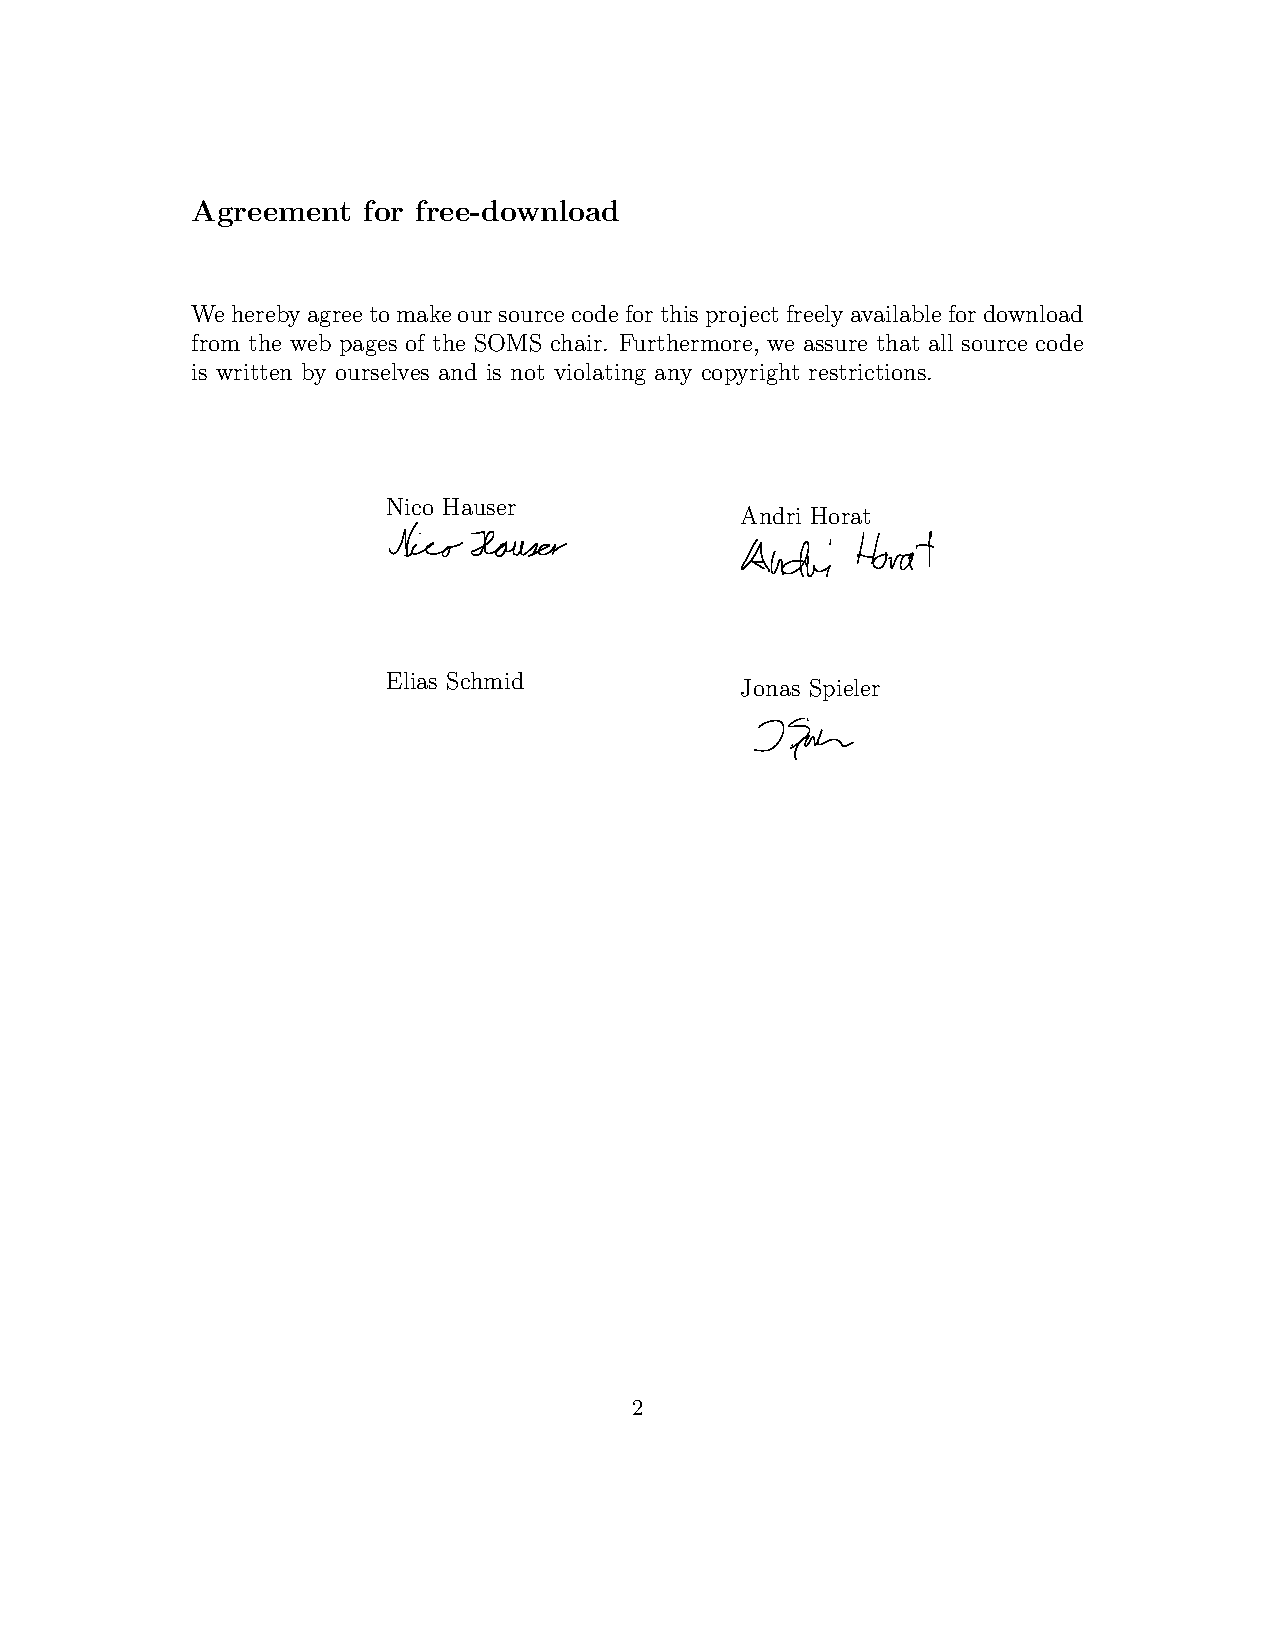
\includepdf[page={1}]{download-agreement}

\newpage

%%%%%%%%%%%%%%%%%%%%%%%%%%%%%%%%%%%%%%%



% IMPORTANT
% you MUST include the ETH declaration of originality here; it is available for download on the course website or at http://www.ethz.ch/faculty/exams/plagiarism/index_EN; it can be printed as pdf and should be filled out in handwriting


%%%%%%%%%% Table of content %%%%%%%%%%%%%%%%%

\tableofcontents

\newpage

%%%%%%%%%%%%%%%%%%%%%%%%%%%%%%%%%%%%%%%



\section{Abstract}

This paper describes a model for the behaviour of people in the event of an emergency situation and it's simulation. The model incorporates the general repulsion of people standing too close, the formation of groups in panic situations, the placement of exit signs and many other factors such as different speeds. In order to make observations on the defined model, it is simulated using a physics engine written in javascript that makes it accessible from any place at any time and allows for reproducible and verifiable results. The paper defines a general parameterised model of the environment and the agents which, with the right choice of simulation parameters, may even allow for a safety evaluation of specific settings. Simulations using this model were able to verify results of other papers but also put them into perspective.

\section{Introduction and Motivations}

This paper was created during the course \textit{Agent-Based Modeling and Social System Simulation} held by Dr. Nino Antulov-Fantulin and Thomas Asikis at ETH Zurich. The goal was to create a project in the field of modelling of complex systems with humans as agents. A complex system is in contrast to complicated system not per se hard to implement but rather consists of many simple small parts that on themselves act based on simple rules. The fact that there are a lot of agents gives rise to behaviours of the whole system that are not always easy to predict or even easy to understand even though it is based on simple rules. As computers keep getting faster and new technology is developed every day, simulations are a good way of understanding these complex systems by playing with the available parameters while looking for emerging patterns and then interpreting the implications for the real world.

\section{Description of the Model}

For the sake of simplicity this chapter is split into the definition of the environment model and the agent model, since the environment model is to some extent independent of the agents model. 

\subsection{Environment model}

Before agents can react to a fire an environment has to be created which in our case is a building. The environment model consists of walls, obstacles, doors and signs all of which are objects the agent interacts with. Walls are the most important part as they give the environment a shape and restrictions to the agent's movements. The same goes for obstacles, the reason why walls and obstacles are separated in our model is that the agent use a raytracing algorithm for finding a path and obstacles such as tables may prevent an agent from moving but do not interfere with their vision. Next are the doors and signs which also have similar roles. As it is the case in real life, safety signs guide an agent to the closest exit where agents are able to escape. Doors have the same effect on agents but represent something different as they're not a physical object but rather represent the agent's memory of where they entered a room. Both signs and doors are directional in our model as both, safety signs and doors, should only be used in one direction when escaping a building.

\subsection{Agent model}
The agent model is implemented as a social force model. In short agents behave like particles in newtonian physics. Every agent has a mass, position and velocity. The intentions and interactions between agents and between them and their environment are represented by forces. An agent is approximated as a circle in the physics engine. Each one is created with different intrinsic properties that are randomly generated using a normal distribution. Some of these parameters are adjustable via the mean value and the standard deviation. The circle diameter of an agent represents the different shoulder widths as it was also done in \cite{Helbing}. In contrast to this paper, we chose the desired velocity from a normal distribution as this seemed more reasonable to us since not every agent in the real world has the same fitness. In addition we also randomly choose a reaction time that determines how fast an agent can change its direction.

After the generation of these random values, the agents are a sole product of their environment and their behaviour is based on a set of simple rules.

\begin{itemize}
    \item Wall repulsion
    
    To model human behaviour, agents should in general prefer to move away from walls as most humans prefer to have some space around them.

    \item Agent repulsion
    
    For the same reason people do not like to stand close to each other, especially not in emergency situations. The closer the distance is, the greater is the applied force on every pair of agents to move away from each other.

%    \item Agent attraction
%    
%    Even though people do not like to stand close to each other, they still tend to form groups and do not like to act on their own. Thus the agents are instructed to move closer together as long as the distance between them is in the acceptable range.

    \item Target attraction
    
    Last but definitely not least the agents need a task. In the best case, they should try to reach one of the defined escape zones in order to safe themselves. In real life, safety signs guide people to these safe zones so the agents are instructed to always be on the lookout for visible signs guiding them to safety, so we do the same in our model and guide agents to the closest visible safety sign or door. In addition agents should remember what signs and doors they have already passed and won't go into the direction of the same sign or door twice. An exception is made to this rule if an agent doesn't have a target anymore. Then they their memory of the visited doors and signs gets cleared and they start from scratch. This allows for some more complex behaviours such as an agent finding again the nearest sign or door after being pushed back into the same room he just had left. If the memory wasn't cleared, the agent wouldn't be able to leave the room a second time which of does not correspond to natural human behaviour.
\end{itemize}

\section{Implementation}

The implementation of this model is done in javascript using a game library called Phaser \cite{Phaser} that already includes a physics engine and has means of drawing the result onto a \texttt{HTML} canvas meaning the whole simulation can easily be rendered on a webpage and doesn't require any setup.

\subsection{Environment construction}
As people are at least to some extent the product of their environment, it is very important that the simulations does not have a fixed environment in which all simulations take place. In fact it is one of the most important parameters when looking at the results, i.e. how many people survived a fire emergency. People in a totally enclosed room have no chance of escaping whereas agents sitting next to an escape zone probably will have no issues. To make the change of this parameter as accessible as possible, the implementation uses an open source format called \texttt{Tiled's map format} (TMX). \cite{Tiled} As the name implies, this format can be edited using the open source editor named Tiled.

\begin{figure}[H]
	\centering
	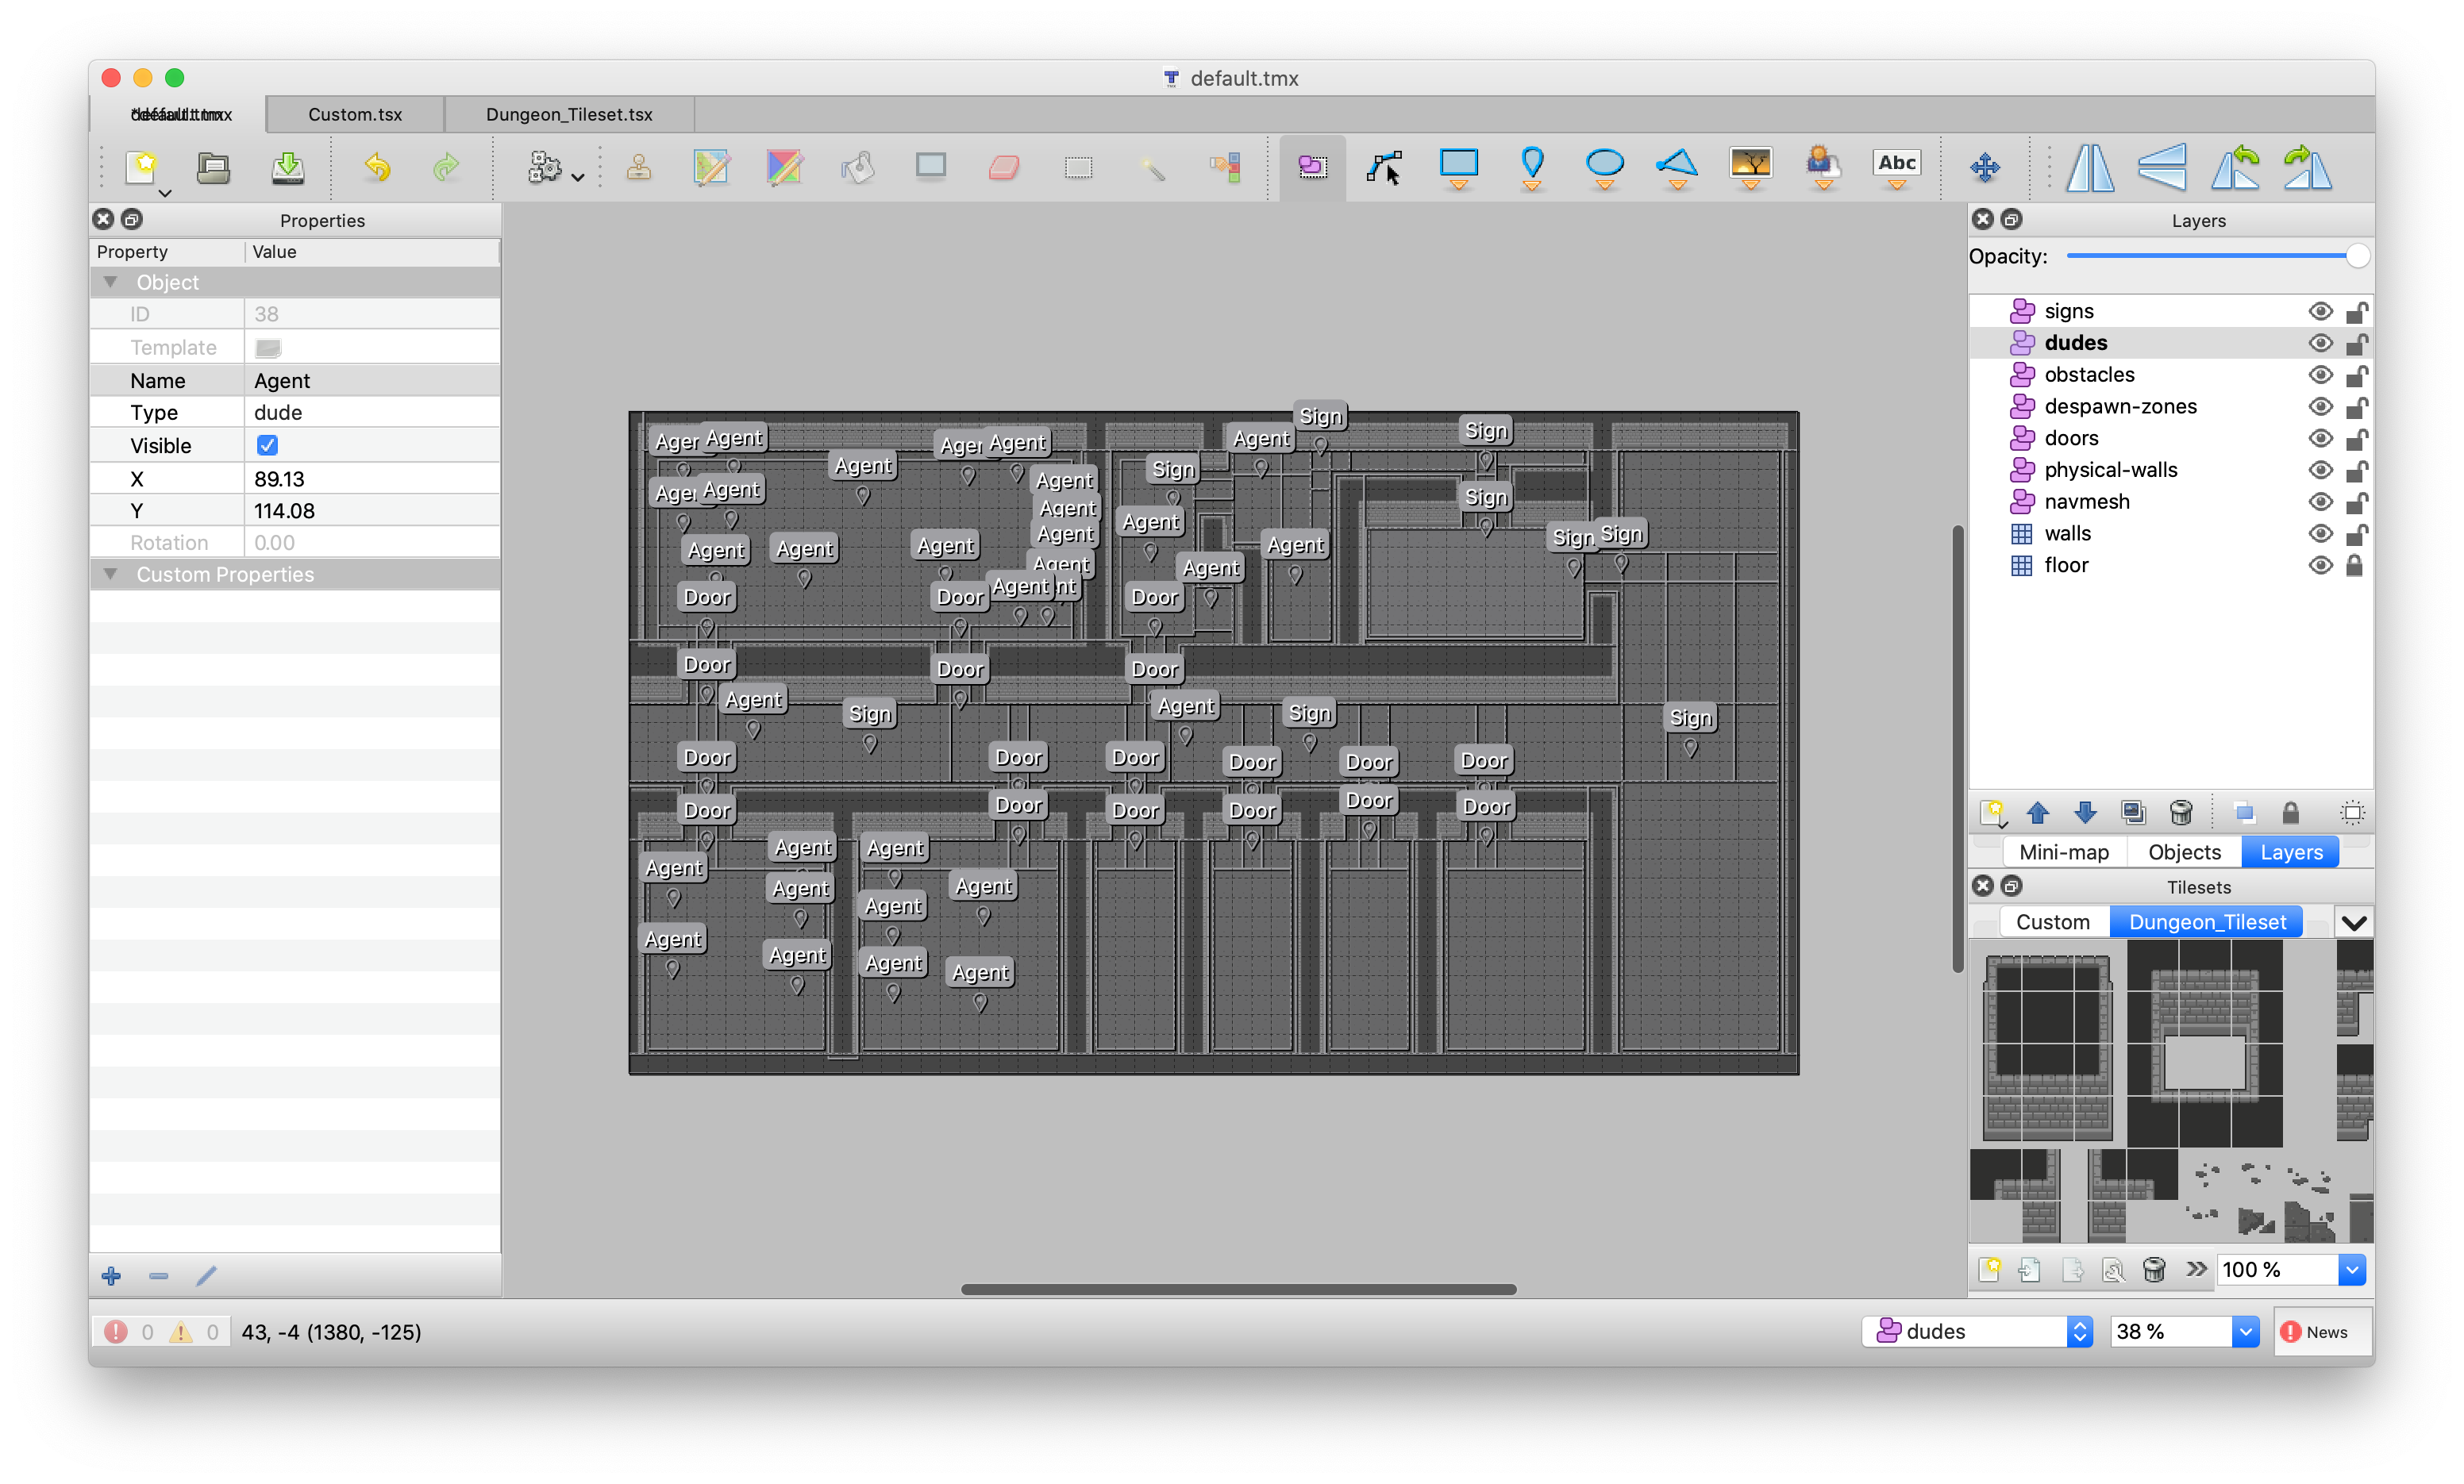
\includegraphics[width=1\linewidth]{assets/tiled-editor}\\
	The editing screen of Tiled \cite{Tiled}
\end{figure}

This editor is very simple to use and everyone with a basic understanding of computer is able to adjust the given examples or to define their own setting. This makes the model much more accessible and allows anyone to fit our model to their own needs and interests.

\subsection{Agent behaviour}

As Phaser includes a physics engine we can make use of this by simulating the behaviour of the agents based on forces acting on them where the resulting movement is the sum over all force vectors. Phaser has an \texttt{update} function that gets called every time a new frame is calculated. which is perfectly suited for a task like our model. The different behavioural rules are implemented as follows

\begin{itemize}
      \item Wall repulsion
    
    The wall repulsion acting on an agent is calculated based on the minimal distance between the agent and all walls. The force pushing the agent away from the wall is defined as
    
    \begin{align*}
    	f_w = c_1 \cdot e^{-\frac{d}{c_2}}
    \end{align*}
 
where $d$ is the vector pointing from the point on the wall to the position of the agent and $c_1$ and $c_2$ are adjustable parameters.

    \item Agent repulsion
    
    Agent repulsion can be implemented rather easily: for every pair of agents there acts a force 
    
    \begin{align*}
    	f_r = c_1 \cdot e^{-\frac{d}{c_2}}
    \end{align*}
    
    pulling them away from each other, where $c_1$ and $c_2$ are adjustable parameters but constant for the two agents. $d$ is the vector difference between the two agents. As the force is proportional to $e^{-d}$, it decreases exponentially with respect to the distance. The initial values for $c_1$ and $c_2$ were empirically determined and are dependent on Phaser's internal units.

%    \item Agent attraction
%    
%    The agent attraction force is, in contrast to the agent repulsion force, linearly dependant on the distance $d$
%    
%    \begin{align*}
%    	f_a = c_3 / d
%    \end{align*}
%    
%    but of course directed in the opposite direction of $f_r$. As $f_r$ is exponentially dependant on $d$ and $f_a$ just linearly there is a distance $d_0$ for which the two forces are in balance and the two agents will stay in place if no other force would act on them.

    \item Target attraction
    
    To verify which signs are visible, we use a technique called raytracing. Our raytracing algorithm works by iterating over all signs and doors and computing if a given sign/door is visible for an agent. This means a line gets drawn from an agent's position to a sign and it gets validated whether this line intersects with a wall defined in the environment. The following part describes some scenarios in which the algorithm works.
    
    \begin{minipage}{.1\textwidth}	
	\vfill\hfill
	\end{minipage}
    \begin{minipage}{.3\textwidth}
		\begin{figure}[H]
		\centering
		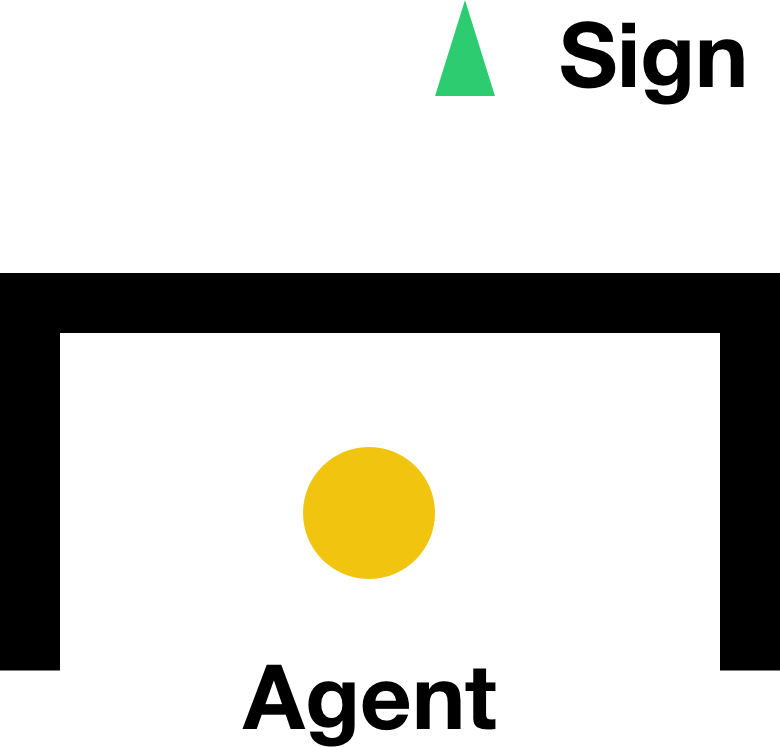
\includegraphics[width=1\linewidth]{assets/raytrace-blocked}\\
		An agent's vision blocked by a wall
	\end{figure}
	\end{minipage}
	\begin{minipage}{.2\textwidth}	
	\vfill\hfill
	\end{minipage}
	\begin{minipage}{.3\textwidth}
		\begin{figure}[H]
		\centering
		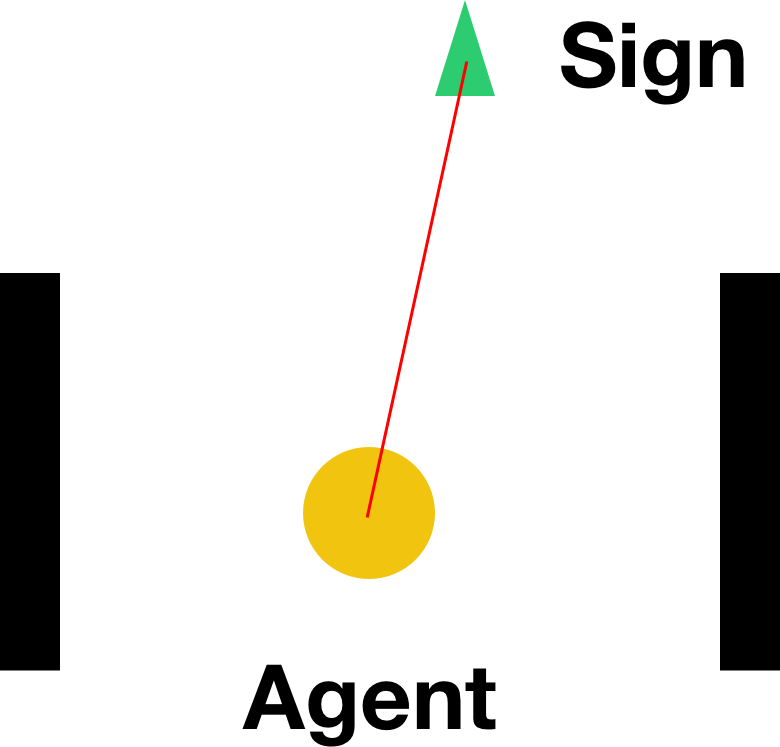
\includegraphics[width=1\linewidth]{assets/raytrace-visible}\\
		An agent's sight of a sign visualized by a red ''ray''
	\end{figure}
	\end{minipage}
    \\\\
	  In the first figure above the agent is surrounded by walls (drawn in black) meaning a line between the agent and the sign would intersect the front wall and thus the agent wouldn't move towards the sign.
    
    If that's not the case, the sign is indeed visible and we can apply a force into the direction of the sign. This works fine until one introduces obstacles (drawn in grey). Obstacles collide with the agent as do walls. The difference is that the agent can see through or over an obstacle and therefore an agent sees a sign or a door behind an obstacle. A good example for obstacle is a table.
	
	\begin{minipage}{.4\textwidth}
		\begin{figure}[H]
			\centering
			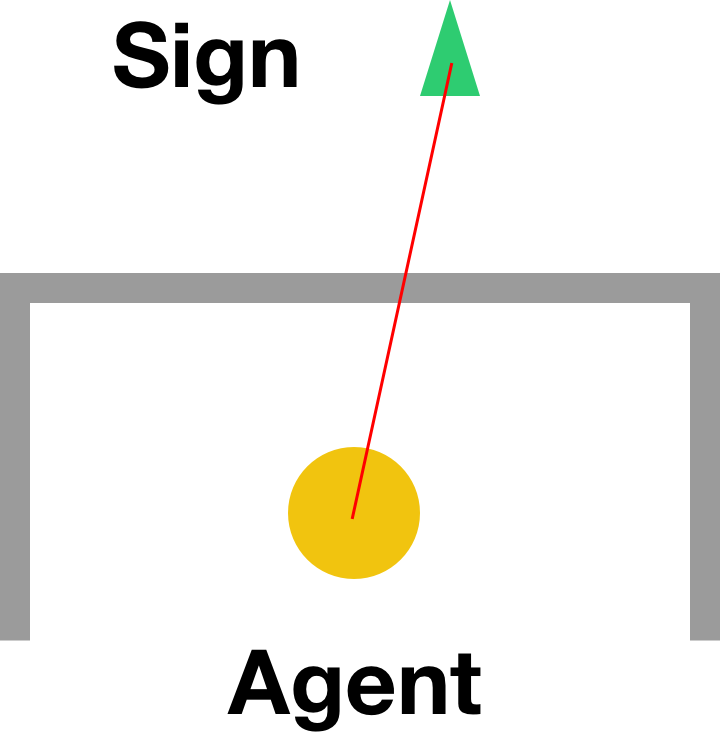
\includegraphics[width=.5\linewidth]{assets/without-navmesh}\\
			Agent stuck within obstacles
		\end{figure}
	\end{minipage}
	\begin{minipage}{.2\textwidth}	
	\vfill\hfill
	\end{minipage}
	\begin{minipage}{.4\textwidth}
		\begin{figure}[H]
			\centering
			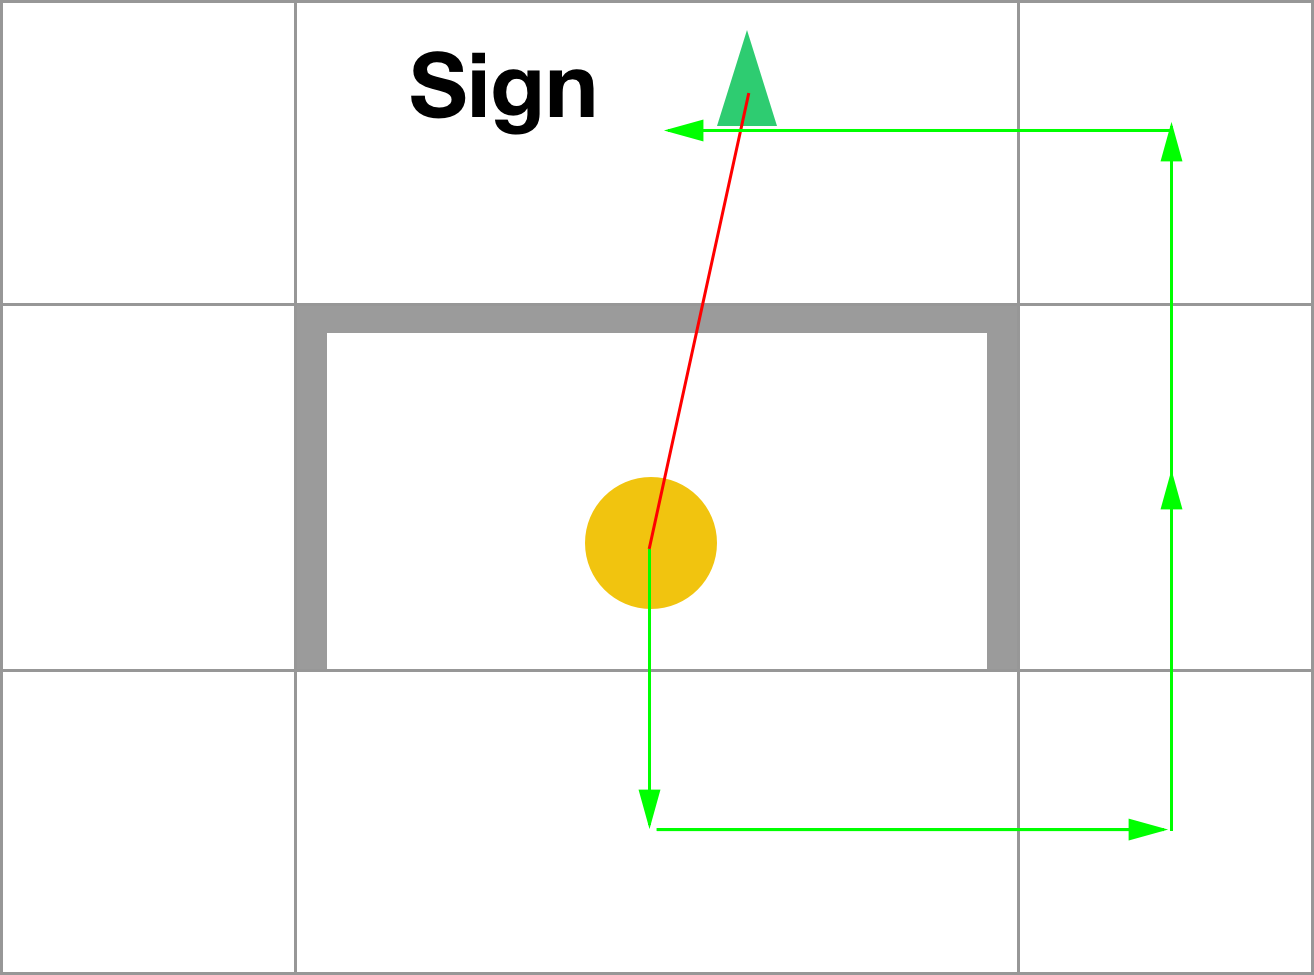
\includegraphics[width=1\linewidth]{assets/with-navmesh}\\
			Agent boxed in obstacles using pathfinding
		\end{figure}
	\end{minipage}
	
	Now the issue with directly applying a force to the agent into the direction of the ray becomes more clear. An agent can get stuck as it cannot move through the obstacle. To circumvent this issue, we take us of a pathfinding algorithm once the agent sees a sign. Now the agent doesn't just move into the targets direction but rather finds a way to the target, surpassing obstacles that lay in their path. The pathfinding algorithm works by generating an ordered list of points that the agent can follow to get from their current position to the target position.
	
	As soon as we know the target of an agent, we can compute the velocity-correcting force, which tries to accelerate the current physical velocity $v_0$ of the agent to the desired velocity $v$. The force gets computed by    
	\begin{align*}
	  f_t = m \cdot \frac{v_0-v}{\tau}
	\end{align*}
	where $m$ and $\tau$ are constants. They can be interpreted as the mass and the reaction time of an agent. In our simulation the $m$ is chosen based on their radius and $\tau$ is a constant defined per agent.
    
\end{itemize}

\section{Simulation Results and Discussion}
To verify our model we tested our tool against an existing paper. We tried to replicate the experiment of first part of the article \textit{Simulating dynamical features of escape panic} \cite{Helbing}. The second experiment was our main purpose of our model, to simulate the stream of agents located in different rooms of a real building. For this case we took a part of the ETH main building.

\subsection{Experiment 1}

For the first experiment we replicated the experiments from the paper \textit{Simulating dynamical features of escape panic} from Dirk Helbing, Illes Farkas and Tamas Vicsek in which the agents had to pass a bottleneck in an escape situation. The conclusion was that there is an optimal velocity of about $1.5 m/s^-1$ at which all 200 agents left in the least amount of time.

\begin{minipage}{.4\textwidth}
		\begin{figure}[H]
			\centering
			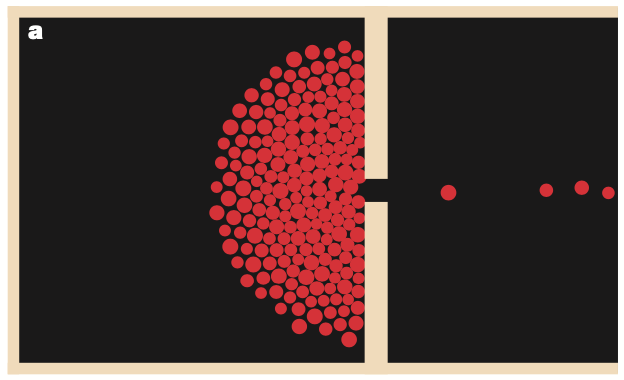
\includegraphics[width=1\linewidth]{assets/helbling-experiment-1}\\
			Setup from \cite{Helbing}
		\end{figure}
	\end{minipage}
	\begin{minipage}{.2\textwidth}	
	\vfill\hfill
	\end{minipage}
	\begin{minipage}{.4\textwidth}
		\begin{figure}[H]
			\centering
			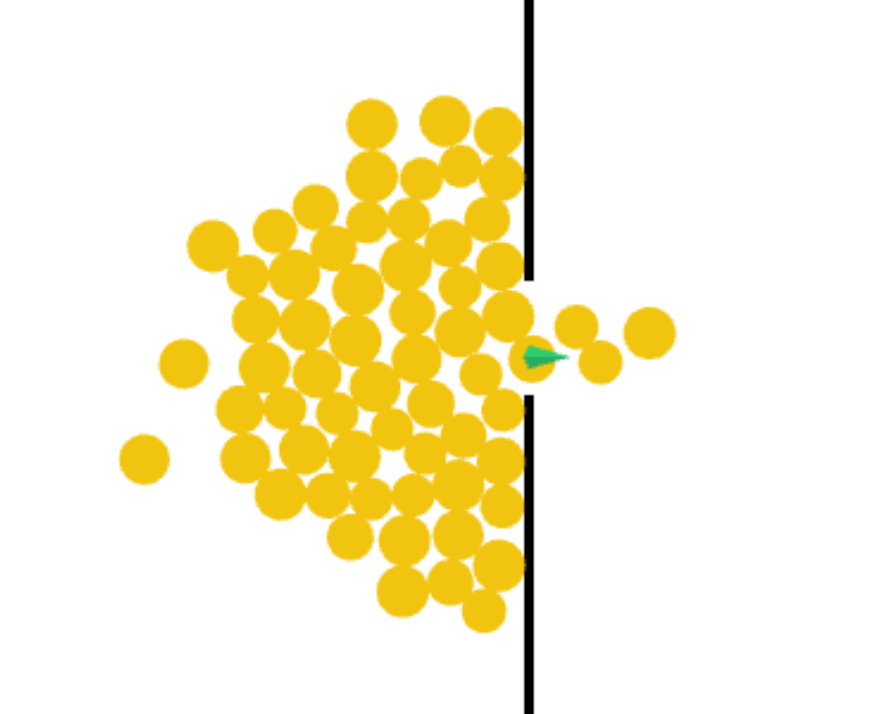
\includegraphics[width=.75\linewidth]{assets/experiment-1}\\
			This paper's setup
		\end{figure}
	\end{minipage}
	
We created a setup similar to that in \cite{Helbing} which is the right image above but in our model this simulation took different turns. When first trying it, some agents started glitching through the wall as the acting forces were extremely high. This is a known issue in physics engines as high forces imply high acceleration and velocity. The path an agent took in a timestep $\delta t$ can be described as $s_1 = s_0 + v\cdot \delta t$.  Since physics engines calculate the new position in discrete time steps without verifying if the path from $s_0$ to $s_1$ could have been taken, glitches like the one described occur. To circumvent this issue, we replaced the whole physics engine with a better one that verifies these cases but also reduced the number of agents. This lead to a new issue that suddenly we couldn't replicate the effect from the paper anymore. Higher velocity almost always resulted in better escape times. When adjusting the friction between the agents this behaviour changed again and now most of the time all agents got stuck in a situation similar to the one described in \cite{Helbing} except that in our case they were stuck indefinitely. As we cannot create statistics where most of the time everyone gets stuck, it prevented us from having a similar statistic as Helbing, Farkas and Vicsek got. When comparing their results with ours, the differences are obvious. Most likely our model failed to replicate some important behaviour that was considered in \cite{Helbing} but it still seems interesting that the paper describes very exactly all parameters chosen for mass, acceleration time, desired velocity, etc. but only mentions the friction very briefly by stating: ''if the friction parameter is large enough''\cite{Helbing}. Depending on how this sentence is interpreted, the results our model produced with a large friction parameter might be more similar than first thought and may also result from a different handling of the friction in the physics engines. For further studies it would be interesting to have a three-dimensional plot with the escape time over the desired velocity and the friction between the agents. Thus the overall question remains, whether a situation visible in the left image above can actually be used in respect to the escape time in real life.

Even though we could not directly verify the results from \cite{Helbing}, the conclusion that higher escape velocities doesn't necessarily result in a shorter escape time could be verified.

\begin{figure}[H]
	\centering
	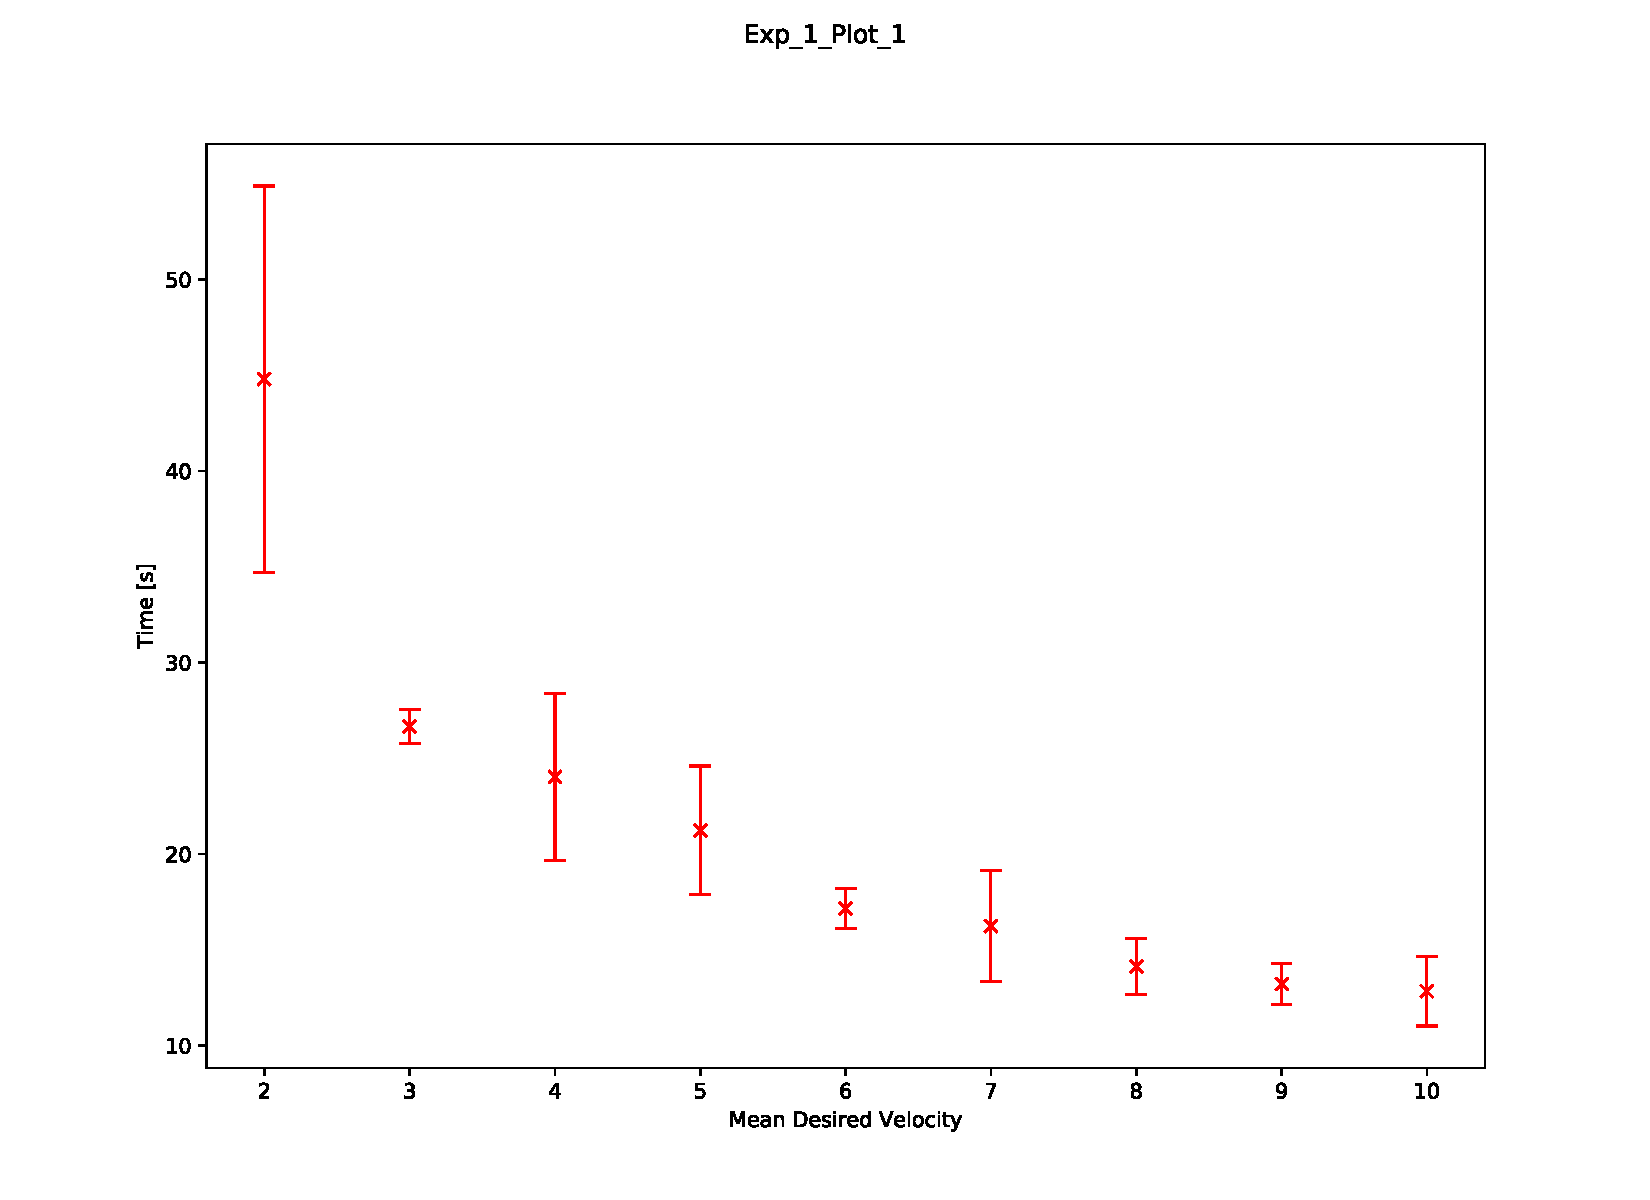
\includegraphics[width=.75\linewidth]{assets/Exp_1_Plot_1}\\
	Escape time over mean desired velocity
\end{figure}

Even though the escape time continuously shrinks with increasing velocity, the difference keeps getting smaller and hits a minimum. In other words a further increase in the desired velocity won't  decrease the escape time as much. This plot is based on five runs per velocity on the described setting.

%\subsection{Experiment 2}

\subsection{Experiment 2}

As our model is capable of handling much more complex situations and complex systems are one of the main topics of the course this paper is written in, we  thought it might be interesting to test the results of the first experiment in a more complex setting. As the environment we chose a simplified version of the ETH Polysnack at noon (1), a modified version with a narrow hallway and a narrow exit (2) and two version in between; one with a narrow hallway and a wide exit (3) and one with a wide hallway and a narrow exit (4).

\begin{minipage}{.5\textwidth}
	\begin{figure}[H]
		\centering
		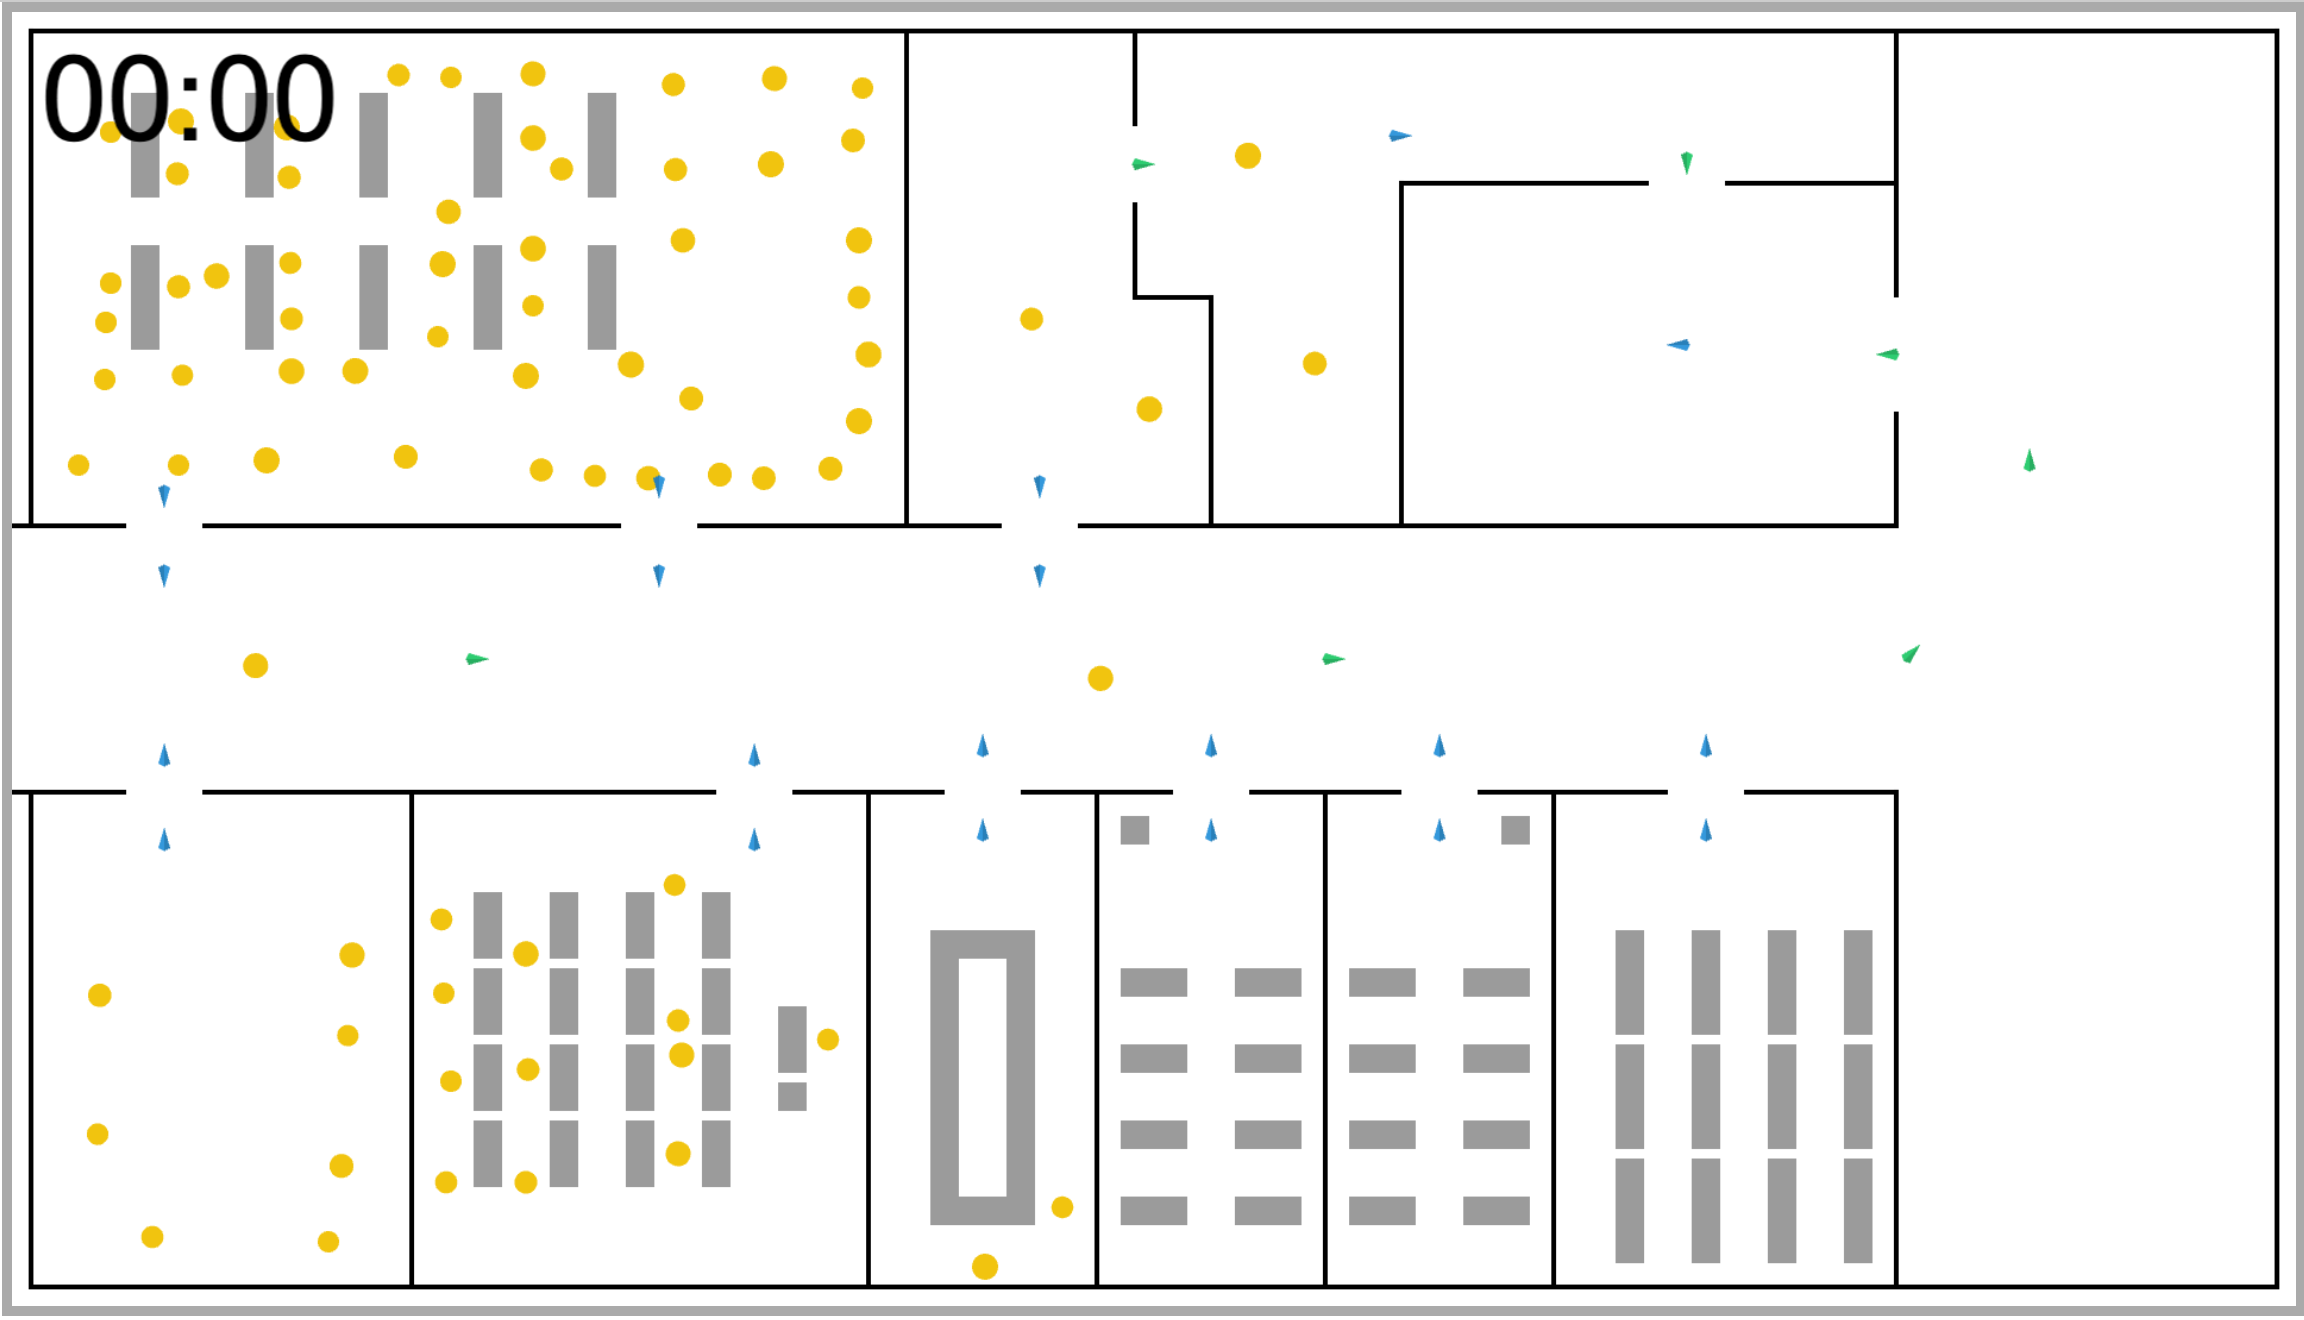
\includegraphics[width=.9\linewidth]{assets/polysnack}\\
		ETH Polysnack
	\end{figure}
\end{minipage}
\begin{minipage}{.5\textwidth}
	\begin{figure}[H]
	\centering
	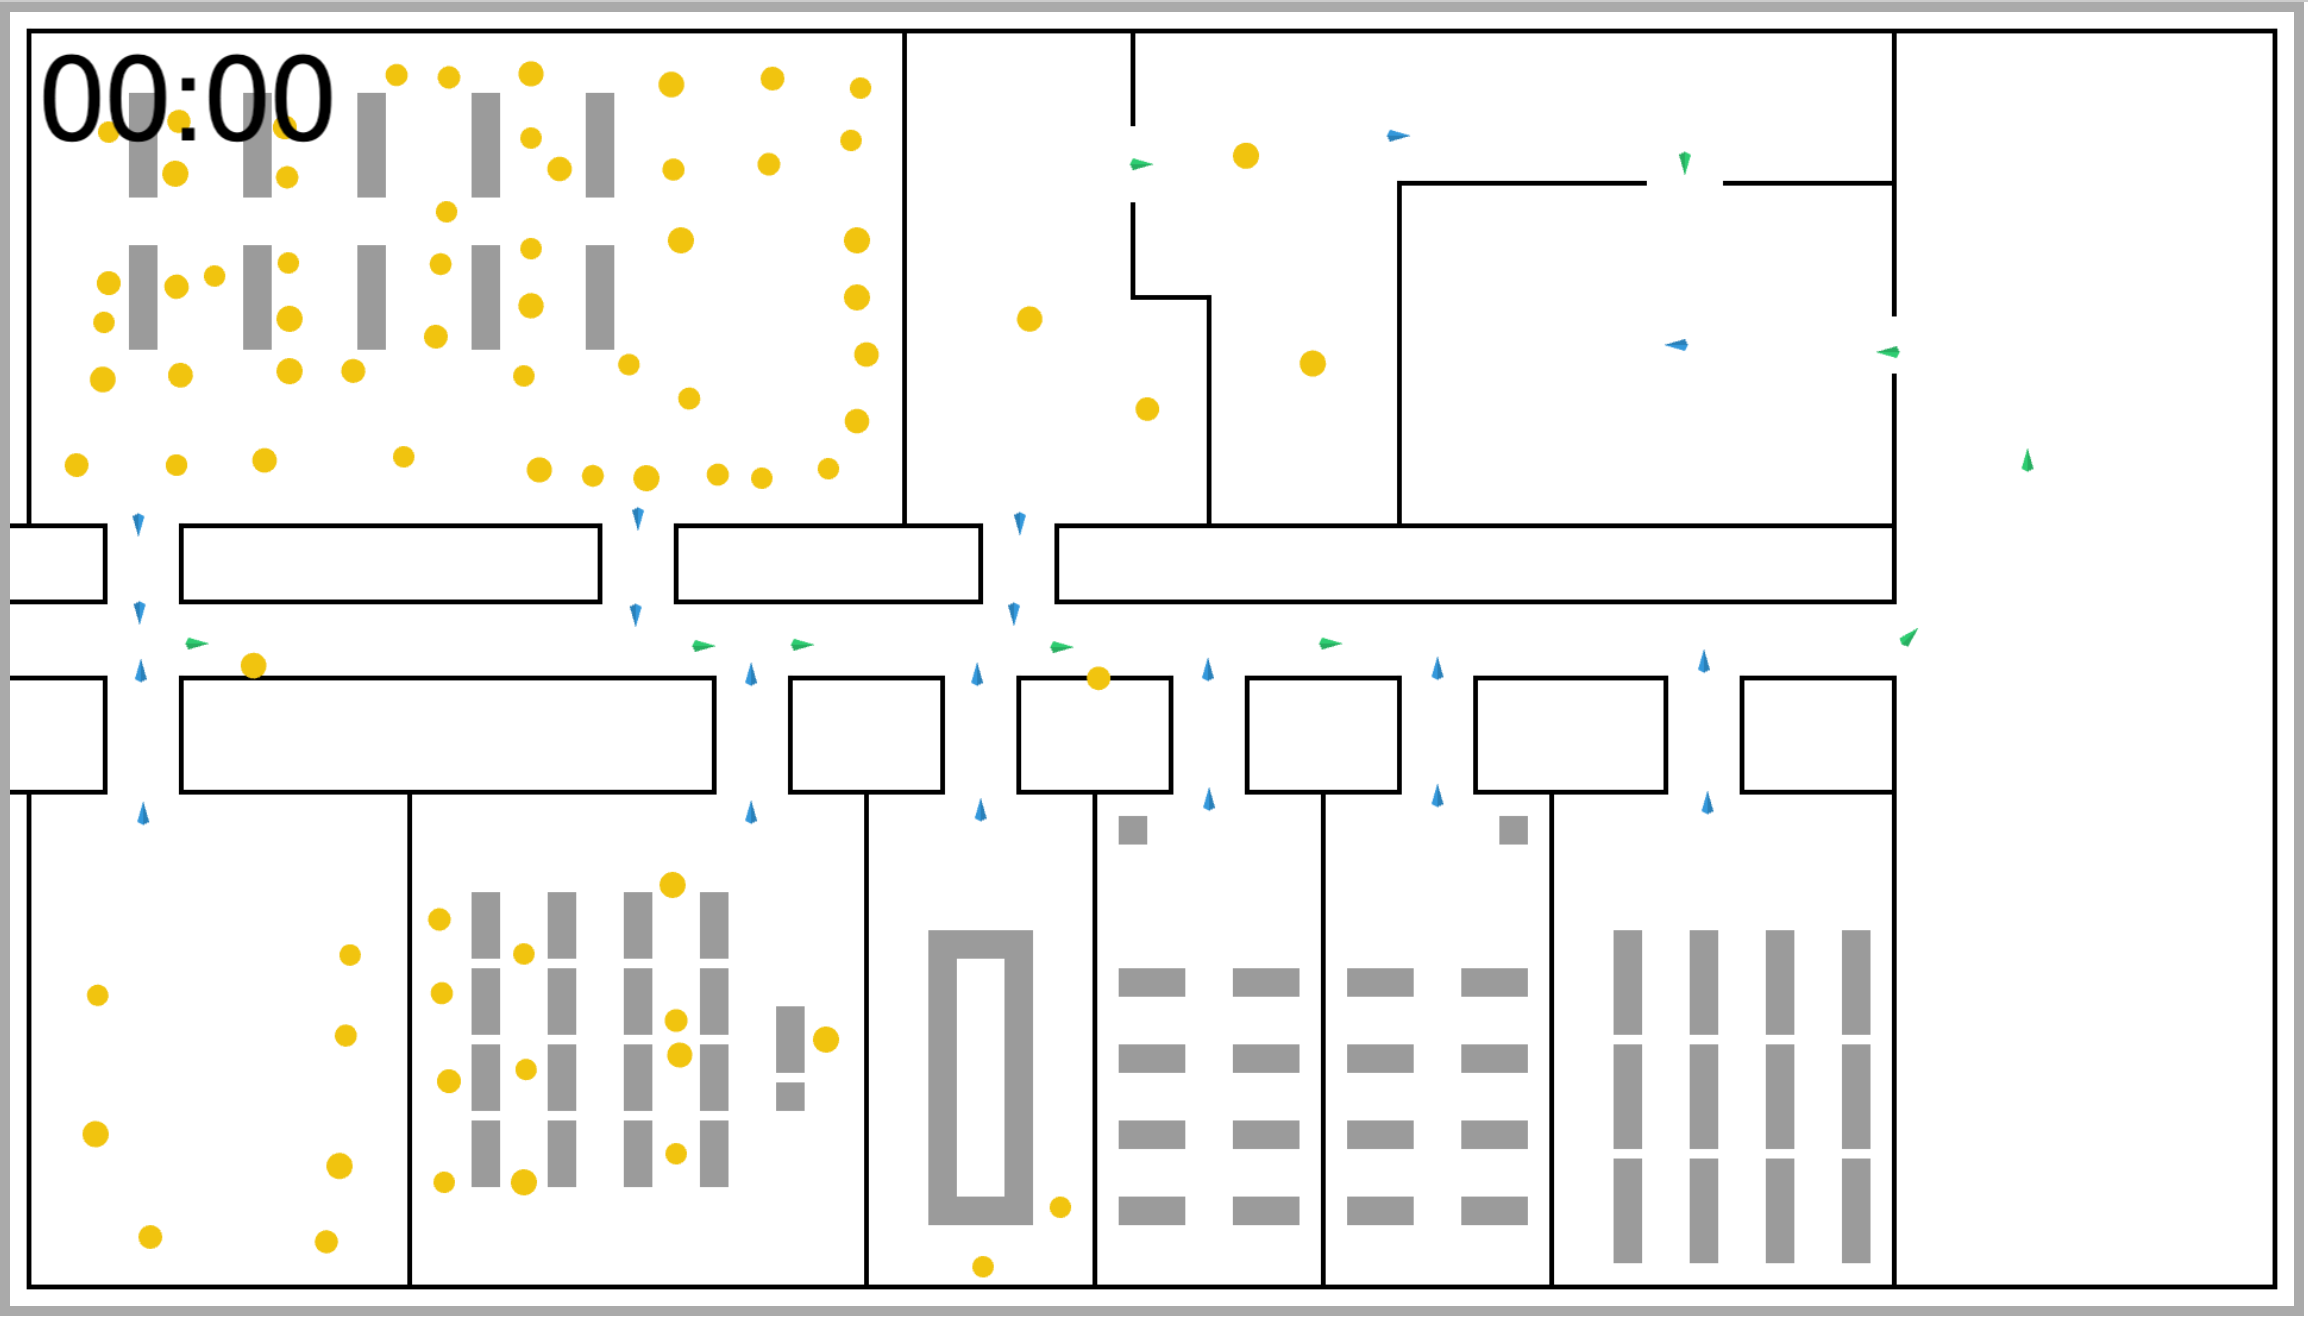
\includegraphics[width=.9\linewidth]{assets/polysnack-modified}\\
	ETH Polysnack with a narrow hallway\\
	and a narrow exit
\end{figure}
\end{minipage}

\begin{minipage}{.5\textwidth}
\begin{figure}[H]
		\centering
		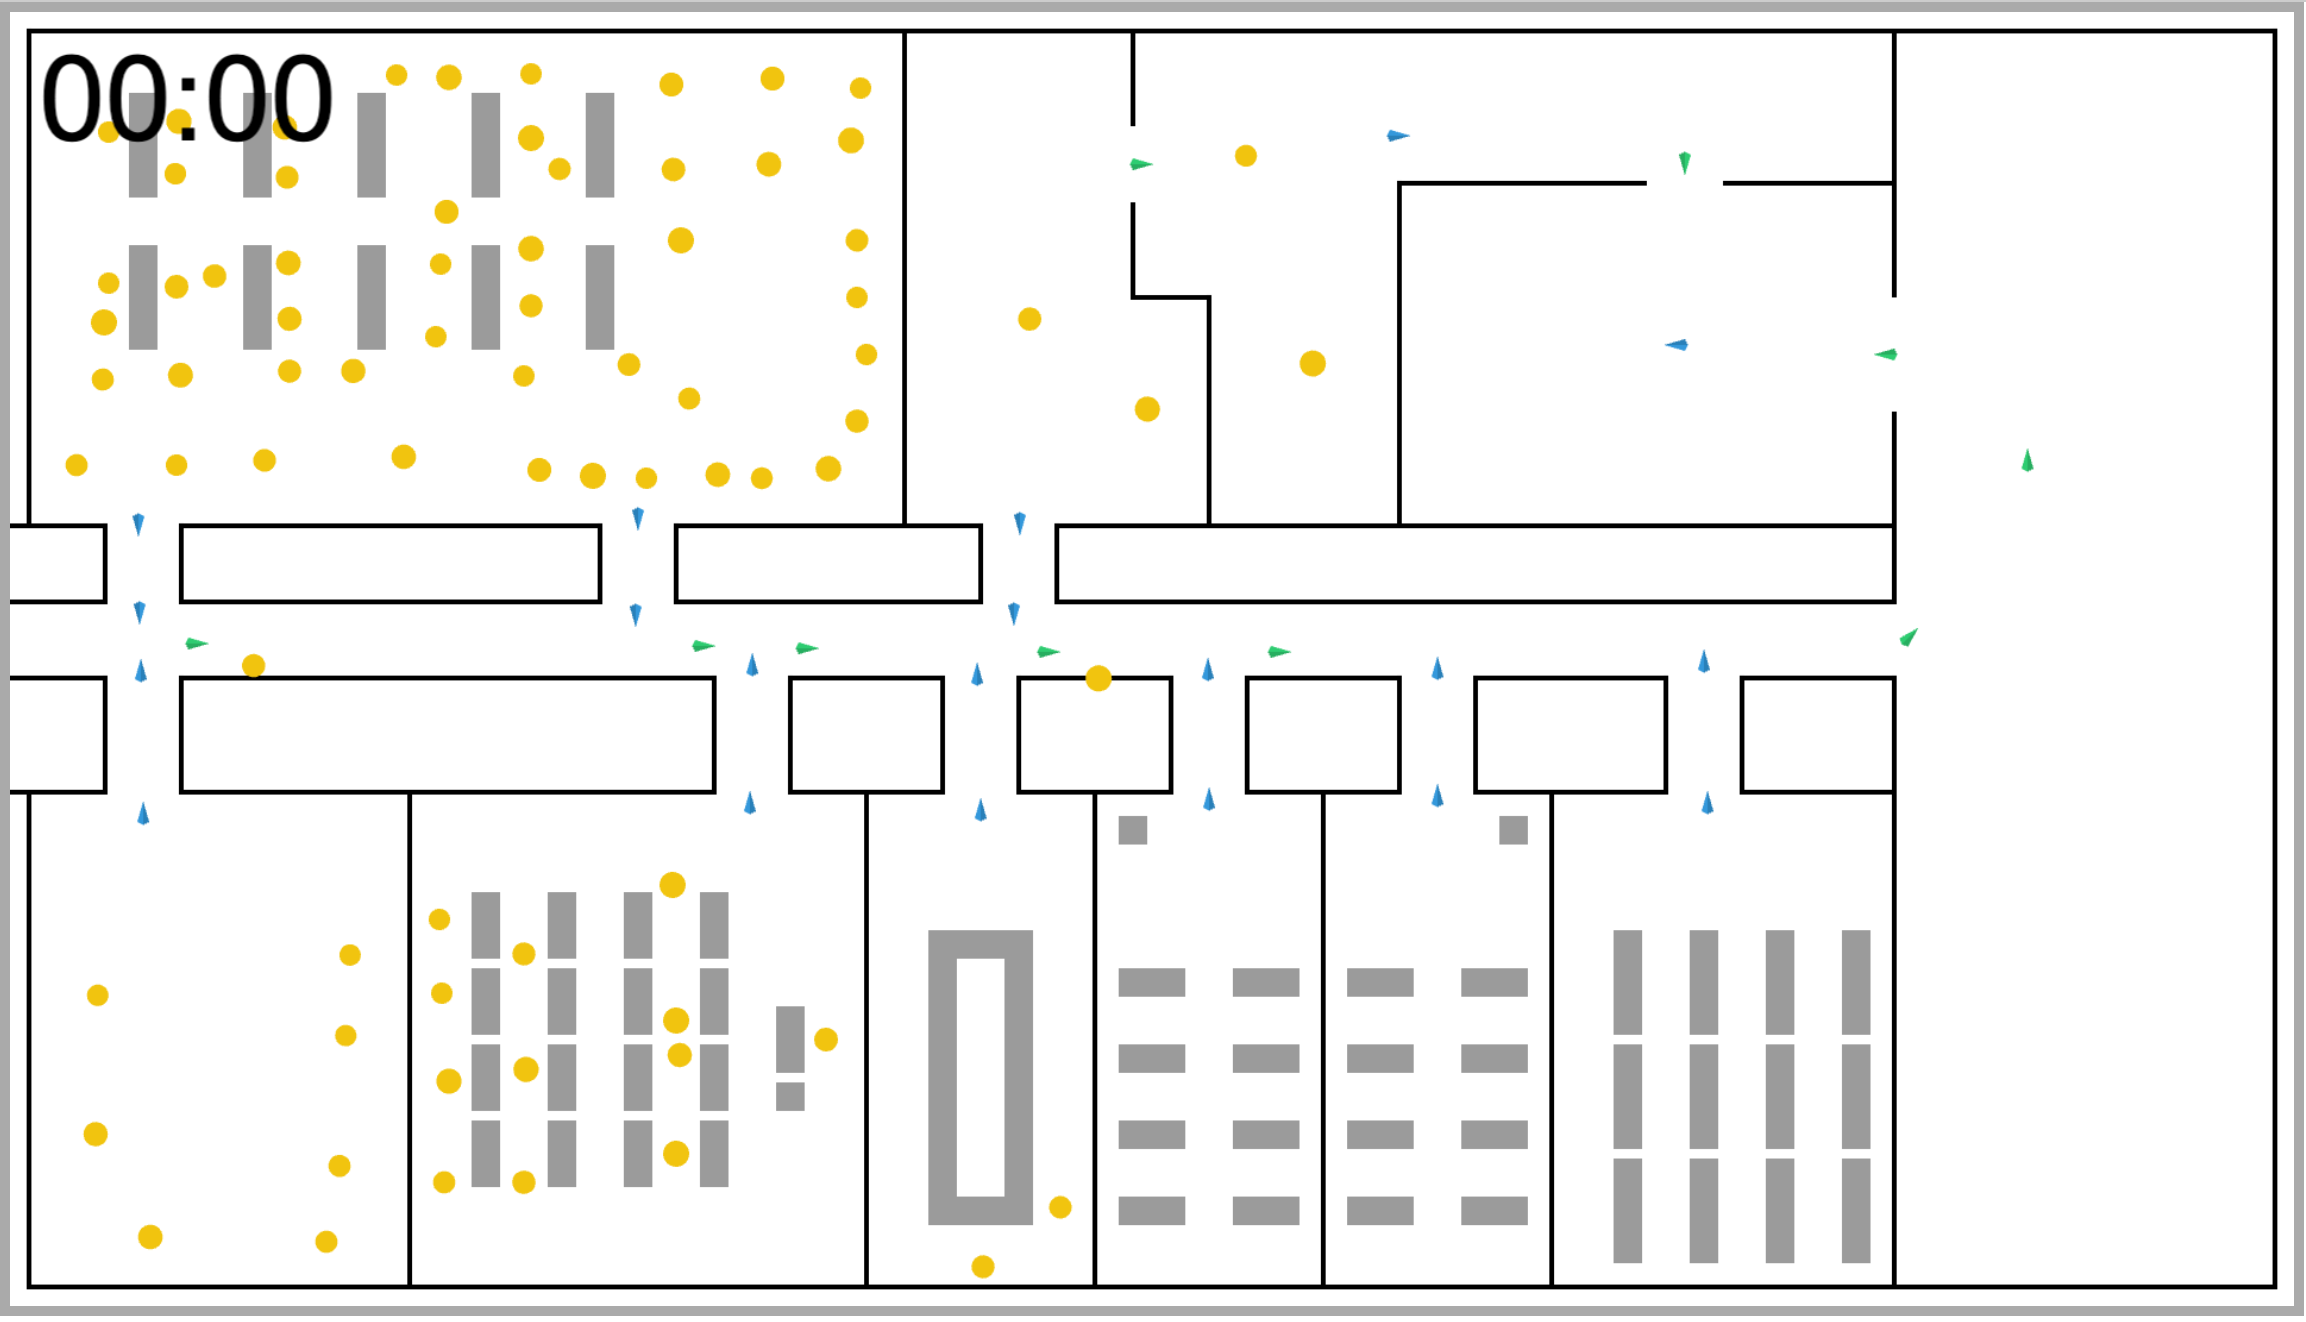
\includegraphics[width=.9\linewidth]{assets/polysnack-experimental}\\
		ETH Polysnack with a narrow hallway\\
		and a narrow exit
	\end{figure}
\end{minipage}
\begin{minipage}{.5\textwidth}
	\begin{figure}[H]
	\centering
	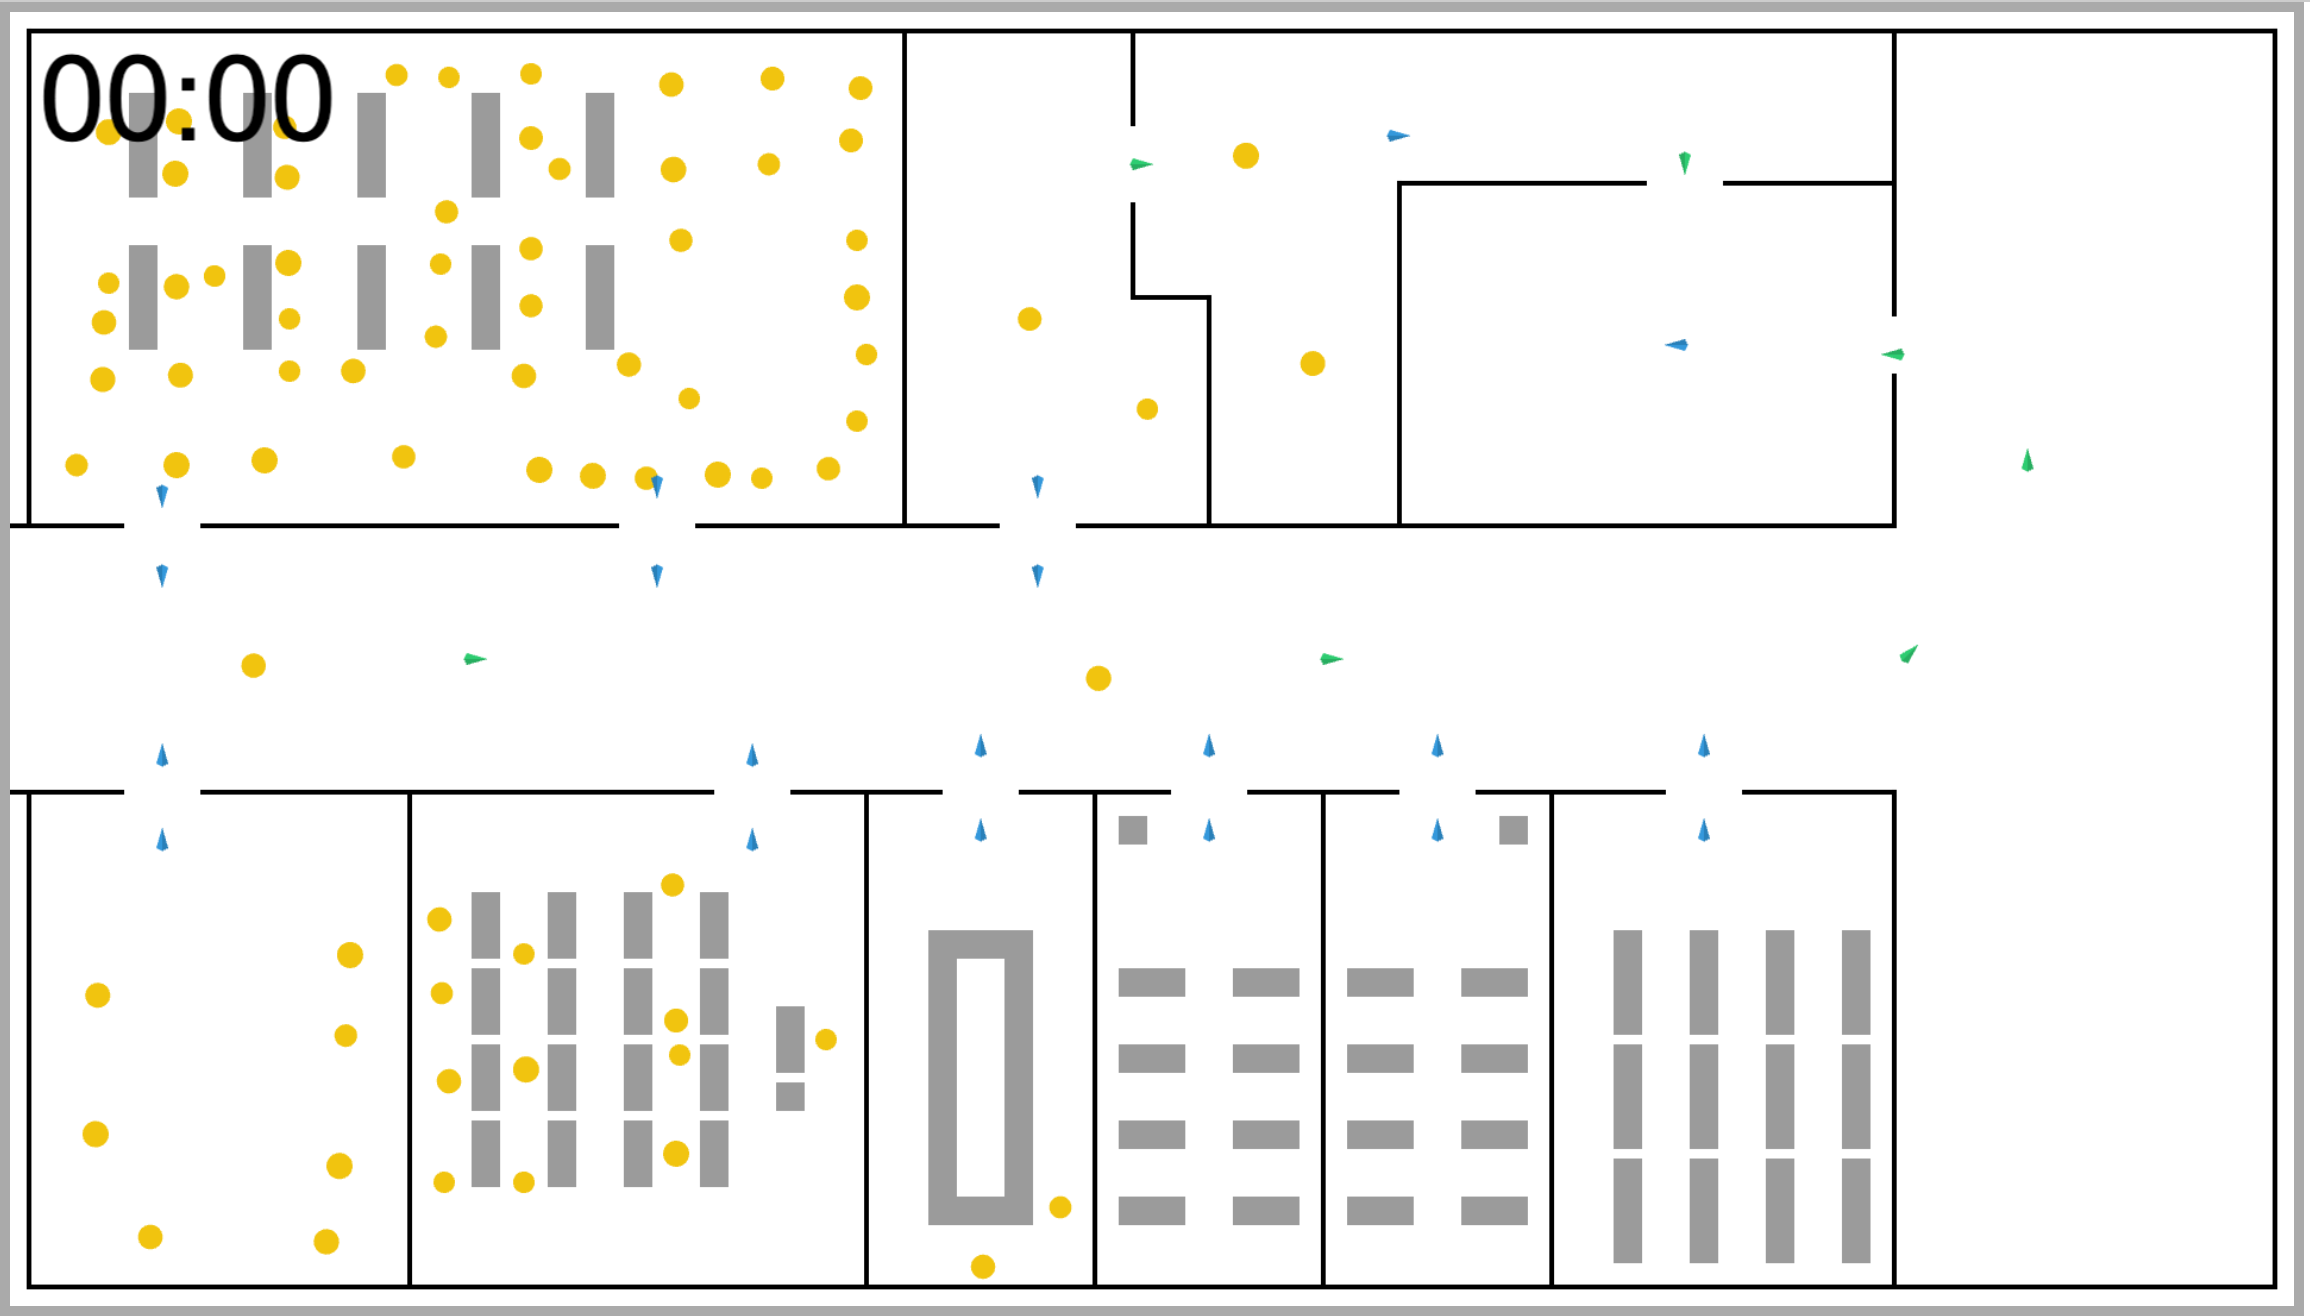
\includegraphics[width=.9\linewidth]{assets/polysnack-experimental-2}\\
	ETH Polysnack with a wide hallway\\
	and a narrow exit
\end{figure}
\end{minipage}

\begin{figure}[H]
	\centering
	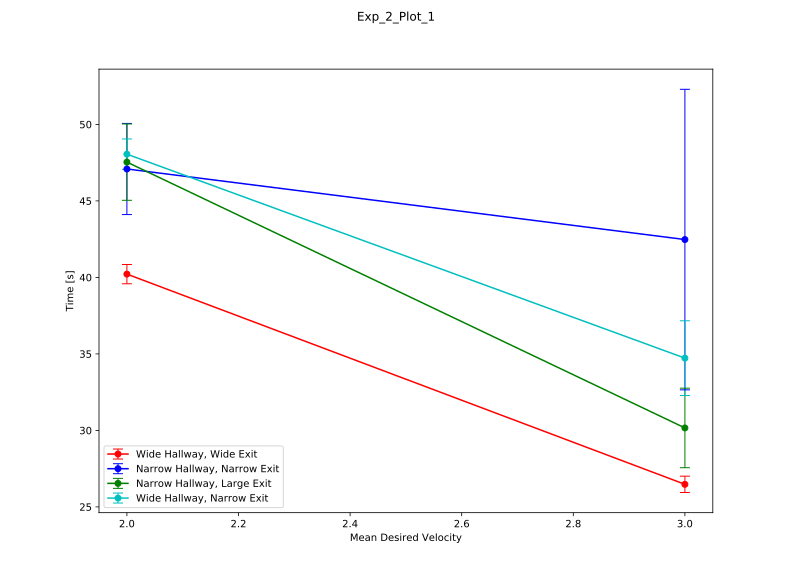
\includegraphics[width=1\linewidth]{assets/Exp_2_Plot_1}\\
	Trend of results of different runs in the three settings
\end{figure}

As expected the first variation has much lower overall escape time than the second variation due to the larger exits and wider hallway. What might be interesting is that the third and fourth variations shown in green and x above, are in between the first two. This might be intuitive to some but before running the experiment one could have also guessed that the wide hallway in combination with the narrow exit might lead to some clogging as the throughput suddenly drops. When visually looking at the progress this actually happens but because the hallway is quite long, the time advantage they get from the long hallway with the larger speed more than compensates for the clogging at the exit. When looking at the statistic above, one can observe a large standard deviation for variation (2) which exactly results from this clogging effect that sometimes takes place. As in our model most initial parameters are chosen from a normal distribution, the results vary much more and thus clogging doesn't happen every time. All in all this might not perfectly judge the whole situation correctly as escape time is just one thing but as mentioned before clogging can result in real bad injuries and is less desirable than being a few seconds faster in a simulation.

%\subsection{Interpretation of the simulation result}
%When running the simulation several times with a range of different parameters, we can observe some similar behaviour as it is already described in other articles.
%
%\subsubsection{Clogging}
%When running the simulation, one might notice that the agents competing for a door are closer together. This is due to the fact, that all agents are pushing towards the door, and hence pushing them together. It worsens the situation, as the friction between the agents increases, which slows down the escape.  
%    
%\subsubsection{Keeping the distance}
%Interestingly, we can observe how agents are pushed back into rooms. Sometimes one could even witness how some agents use another path to avoid the crowd. This is actually what we would expect because of the mutual repulsion of the agents. 
%
%\subsubsection{'Faster-is-Slower effect'}
%There are already many published papers regarding the social-force-model. Of which many describe the 'Faster-is-Slower effect' \cite{Helbing, Wang}. The 'Faster-is-Slower effect' describes the phenomenon where the escape through an exit door is slower if the agents are pushing harder. When running our simulation on our default map, we did not observe this effect. The chances are, that this is due to the long corridor, where the agents make up time with a higher speed.
%
%\subsection{Adapting the parameters for better results}
%
\subsection{Model evaluation}

\subsubsection{Evaluation of the building model}
The building model seems pretty solid and wasn't really an issue during our simulations. Also the possibility of having a graphical editor is very handy. Depending on the emergency situation it might be interesting to extend the building model to support fire, smoke or maliciously acting agents such as terrorists. A lot of work was already done in supporting fire, smoke and their impact on sight is accessible when working with the code but it wasn't used in any experiment as the features weren't stable in time.

\subsubsection{Evaluation of the agent model}
The agent model on the other hand isn't perfect to say the least. It served the simulations pretty well and the graphical results were mostly nice too look at but the social force model has it's limitations. We tried to circumvent some of these limitations with additional raytracing and pathfinding algorithms but the result wasn't perfect. Also there are a lot of undefined parameters in our simulation that weren't fixed to a specific value because of some analysis other than our empirical analysis of what works and what not. The underlying physics engine supports much more that could be made use of but as time was limited it wasn't possible within the scope of this paper. In addition, tracking the forces on the human body and simulating agents falling over would be necessary to model an emergency situation better, especially if clogging takes place. Also the repulsion force between the agents should only apply if the two agents actually see each as otherwise two people standing next to the same wall but in two different rooms will have a pretty strong forces acting on them which of course doesn't represent the reality accurately. For this to be possible, the performance of the raytracing implementation would have to be improved as it would run $O(n^2)$ times every frame (where $n$ is the number of agents). Further improvements would be a force representing the agent's urge to build groups and follow other people. Part of this was already implemented but also wasn't finished in time so it couldn't be used in the final experiments.

%The target attraction probably could have been modelled in a better way, instead of simply applying a force into the direction of the target, a real pathfinding algorithm could try to find the fastest way to the target that may involve walking around obstacles. In the current implementation agents fail to walk to the target if they are boxed in into the direction of the target.

\section{Summary and Outlook}
Even though the experiments didn't yield the results we had hoped for, one can draw interesting conclusion from them and they show where such a social force model reaches its limits. What definitely is different in this project compared to many others is the reproducibility, we really like the idea of having a simulation that can be run right in the web browser and thus the experiments are easily verifiable by others. One mistake we did as a group was to focus too much time on the model itself. As none of us had a lot of experience in building a solid social system simulation, it took us way too long to implement it in a way we were confident with. In the end agents just are simulated particles in newtonian physics but we wanted to actually build a good model for simulating real people which made us implement everything several times and thus wasting time. Just the map format itself was revised at least ten times! But in conclusion one can say that the modelling and the simulation of this scenario was very fascinating and a lot of fun for everyone involved. Even though many ideas were already mention in the chapter about the model evaluation, we would like to mention that the model could further be improved to support many of the things we mentioned, the resource that was preventing us from doing it was in the end just time. One could start building this simulation more accurately, maybe even in proportions to actual SI units, one could improve the performance of the raytracing algorithm and ensure the agents only act repulsive forces on each other if they actually see each other and one could finish implementing one of the many planned features such as fires, smoke or group formation. But still, we're proud of what we built and hope this project can be used by others and will be further developed.

%\section{References}

%To add references, search the paper on https://www.researchgate.net/publication/12295370_Simulating_Dynamic_Features_of_Escape_Panic/citation/download
% and then copy the BibTeX Citation into the file refs.bib

\bibliographystyle{plain}
\bibliography{refs}

\newpage


\includepdf[page={1}]{declaration-originality}

\end{document}  



 
